\documentclass[conference]{IEEEtran}
\IEEEoverridecommandlockouts
\usepackage{cite}
\usepackage{amsmath,amssymb,amsfonts}
\usepackage{textcomp}
\usepackage{xcolor}
\usepackage{enumitem}
\usepackage{calc}
\usepackage{float}
\usepackage[colorlinks=true,urlcolor=blue,linkcolor=green]{hyperref}
\usepackage{graphicx,svg}
\svgsetup{inkscapelatex=false,inkscapepath=./build/svg-inkscape}
\svgpath{{images/}}
\graphicspath{{images/}}

\usepackage{lipsum}

\def\BibTeX{{\rm B\kern-.05em{\sc i\kern-.025em b}\kern-.08em T\kern-.1667em\lower.7ex\hbox{E}\kern-.125emX}}
    
\begin{document}

\title{Medify -- A medication reminder Android App}

\author{\IEEEauthorblockN{Ekrem Emre}
\IEEEauthorblockA{\textit{HTWG Konstanz -- University of Applied Sciences, Germany} \\
\textit{Matriculation number: 302110} \\
ek741emr@htwg-konstanz.de}
}

\maketitle

\begin{abstract}
\lipsum[1][1-4] %TODO
\end{abstract}

\section{Introduction}
\lipsum[2][1-10] %TODO

\section{Goal of the project}
\lipsum[3][1-13] %TODO

\section{Requirement analysis}

\subsection{Personas}
To simulate users for this application, two personas were created, which represents the user types
that might us this application.

\subsubsection{First persona} \hfill
\begin{figure}[h]
	\centerline{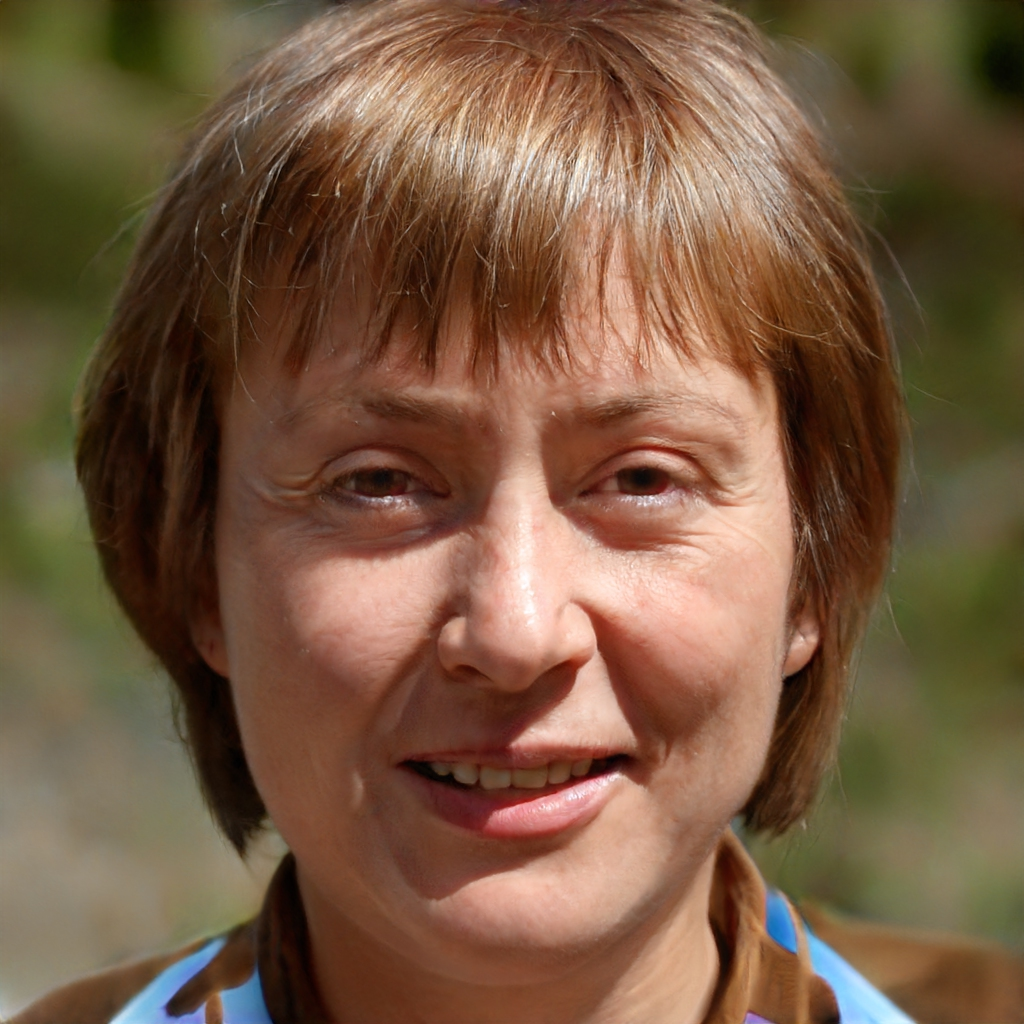
\includegraphics[width=.5\linewidth]{images/persona01.jpg}}
	\caption[Portrait of the persona Rosalyn Foster; Source taken from \cite{personaimg}.]
	{\tabular[t]{@{}l@{}}Portrait of the persona Rosalyn Foster.\\ Source taken from \cite{personaimg}.\endtabular}
	\label{fig:persona1}
\end{figure}

\begin{description}[labelwidth=\widthof{\bfseries Computer skills},leftmargin=.8cm,labelindent=.8cm]
	\item[Name] Rosalyn Foster
	\item[Age] 68
	\item[Marital status] Married
	\item[Occupation] Retiree
	\item[Computer skills] poor
\end{description}

\paragraph*{Key characteristics}
\begin{itemize}[leftmargin=1.25cm]
	\item Retiree, former tailor.
	\item Because of her advanced age, she got forgetful.
	\item Is regularly taking different medication, which she needs to be reminded of.
	\item Is concerned about her health, because she just became a grandparent and wants to spent as much time as possible with her grandchildren.
\end{itemize}

\paragraph*{Goals}
\begin{itemize}[leftmargin=1.25cm]
	\item Be healthy.
	\item Remember taking her medication regularly.
\end{itemize}

\paragraph*{User story}
As an older person, Rosalyn wants to be reminded to take her medicine, because she forgets them and wants to get healthy.

\subsubsection{Second persona} \hfill
\begin{figure}[h]
	\centerline{
\includegraphics[width=.5\linewidth]{images/persona02.jpg}}
	\caption[Portrait of the persona Christian Metz; Source taken from \cite{personaimg}.]
	{\tabular[t]{@{}l@{}}Portrait of the persona Christian Metz.\\ Source taken from \cite{personaimg}.\endtabular}
	\label{fig:persona2}
\end{figure}

\begin{description}[labelwidth=\widthof{\bfseries Computer skills},leftmargin=.8cm,labelindent=.8cm]
	\item[Name] Christian Metz
	\item[Age] 32
	\item[Marital status] Engaged
	\item[Occupation] Physiotherapist
	\item[Computer skills] strong
\end{description}

\paragraph*{Key characteristics}
\begin{itemize}[leftmargin=1.25cm]
	\item Working as a physiotherapist and doing a lot of sports, therefore is very healthy.
	\item He's a member in several sport clubs and a volunteer in the local animal shelter.
	\item His schedule is always pretty full and he's always on the go.
	\item He wants to increase his health by taking some vitamins, because he suspects he has some deficiencies.
\end{itemize}

\paragraph*{Goals}
\begin{itemize}[leftmargin=1.25cm]
	\item Be reminded, to take his vitamins.

\end{itemize}

\paragraph*{User story}
As a healthy person, Christian wants to be reminded to take his vitamins, because he's busy all day and not thinking of it and wants to stay healthy.

\subsubsection{Summary}
These personas show a user group, which are in need to take medication. However they struggle to 
remind themselves to take them in their daily lives.

\subsection{Storyboards}
\begin{figure*}
	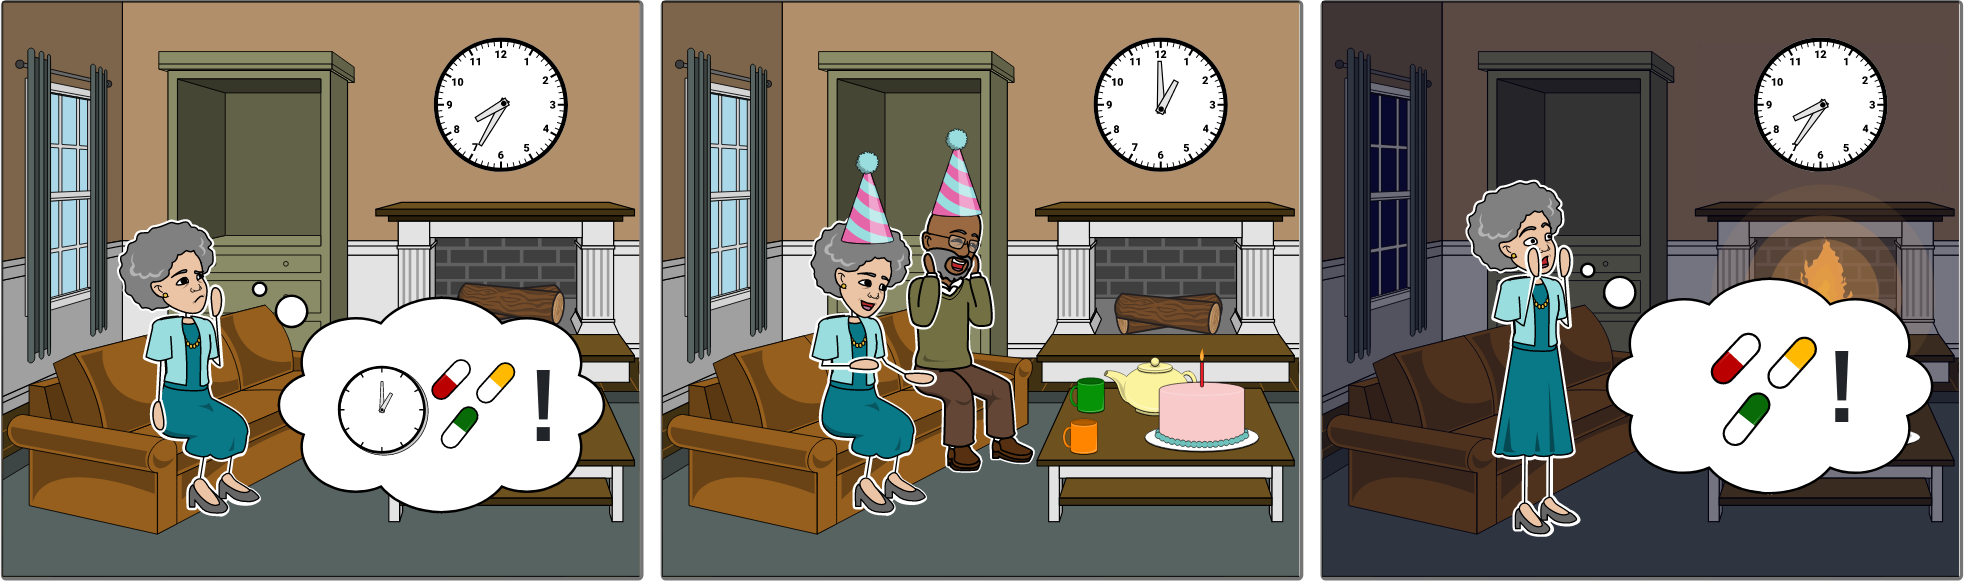
\includegraphics[width=\linewidth]{images/storyboard01.png}
	\caption
	{Storyboard showing an elderly person on her daily activities.
		In the first panel she reminds herself to take her medication at one o'clock.
		The second panel shows her enjoying her day with a friend, however she forgets to take her medicine.
		The last panel shows her in the evening and she realizes her blunder.
		Graphic created using \cite{storyboard}.}
	\label{fig:storyboard1}
\end{figure*}

\begin{figure*}
	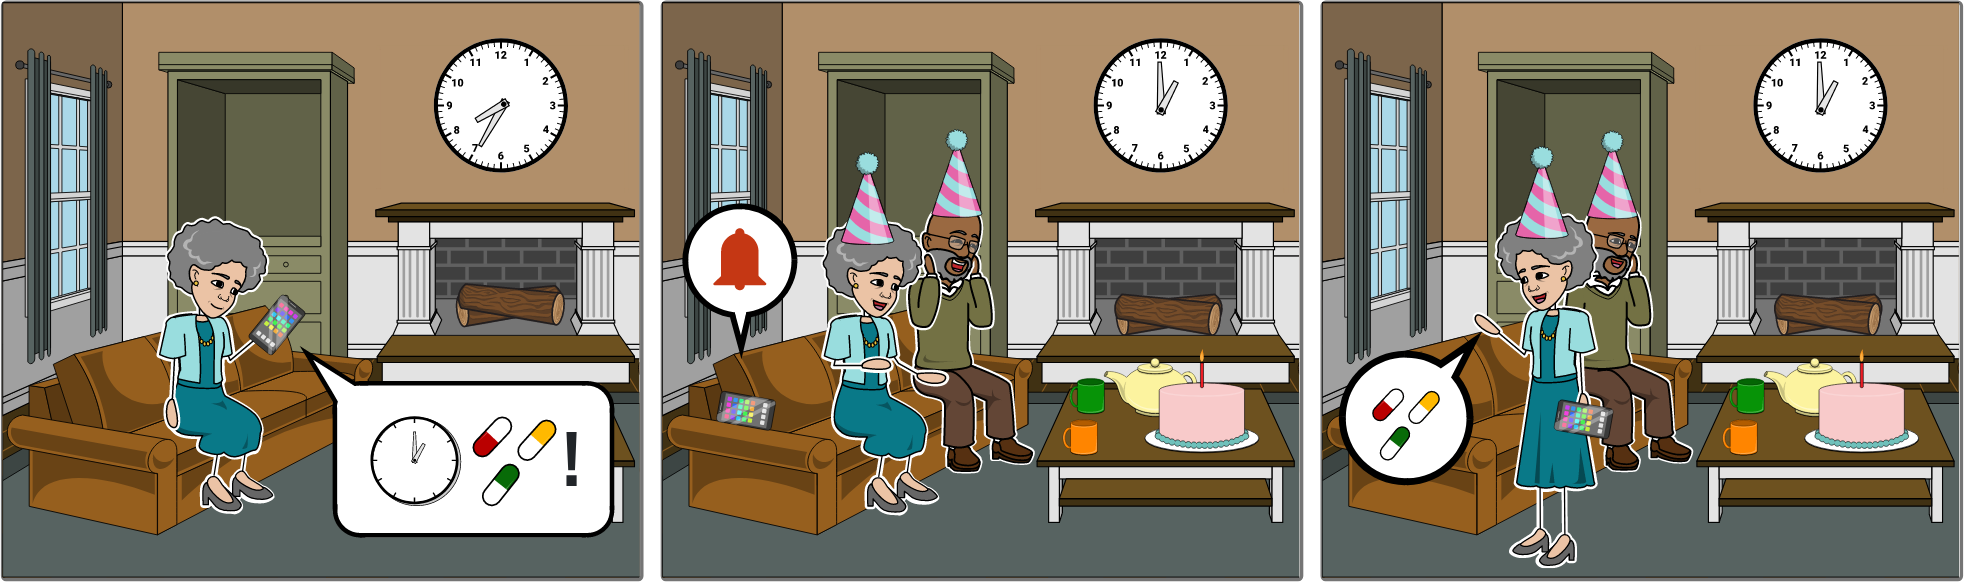
\includegraphics[width=\textwidth]{images/storyboard02.png}
	\caption
	{Storyboard showing an elderly person on her daily activities while using a medication reminder application.
		In the first panel she sets an alert on her smartphone, using the medication reminder app, at one o'clock.
		The second panel shows her and a friend enjoying their day. The medication reminder app alerts her at the set time, to take her medication.
		In the last panel she picks up her phone and takes her medication, just as advised by the application.
		Graphic created using \cite{storyboard}.}
	\label{fig:storyboard2}
\end{figure*}

To illustrate the practical use of a medication reminder application a storyboard was designed.
Fig. \ref{fig:storyboard1} shows an elderly person, which after some distractions in her daily
routine forgets to take her medicine.
Fig. \ref{fig:storyboard2} shows the same elderly person in a similar scenario. In order to manage
her medication, she uses her smartphone to get reminded when to take her medicine.

\subsection{Summary}
The requirement analysis shows, that the application must be capable of reminding the user when to take
their medicine. The time of notification shall be set by the user. In order to accommodate users who need
to take different medications at different points in time, the application shall be able to record multiple
medications with multiple alerts.

In order to facilitate the usage of the application, it shall include a way to scan GTIN/EAN--labels and
autonomously recognize the name of the scanned medication.

\section{Conceptual model of the solution}

\subsection{Entity relationship diagram}

\begin{figure}[H]
	\centerline{\includesvg[width=\linewidth]{entity_relationship_diagram}}
	\caption{Entity relationship diagram to depict the data model.}
	\label{fig:entity_relationship_diagram}
\end{figure}

Fig. \ref{fig:entity_relationship_diagram} shows a entity relationship diagram of the application.
Two entities emerged when designing a first solution. \texttt{Medication} has the attributes \texttt{name},
\texttt{description} and a \texttt{1:n} relationship to \texttt{AlertTimestamp}, which has \texttt{timestamps}.
By designing the data model this way, it is possible to have multiple \texttt{Medication}-entries associated with multiple different \texttt{AlertTimestamp}-entries.

\subsection{Activity diagram}

\begin{figure}[H]
	\centerline{\includesvg[width=\linewidth]{activity_diagram}}
	\caption{Activity diagram showing the main workflow of the application.}
	\label{fig:activity_diagram}
\end{figure}

Fig. \ref{fig:activity_diagram} shows the workflow of the application. Beside the basic \textit{CRUD} operations
to the database, actions for scheduling reminders and fetching data from a remote \textit{API} included. In order
to keep this diagram plain, the scheduling and \textit{API} actions are deliberately kept simple.

\subsection{Mockups}

\begin{figure}[H]
	\centerline{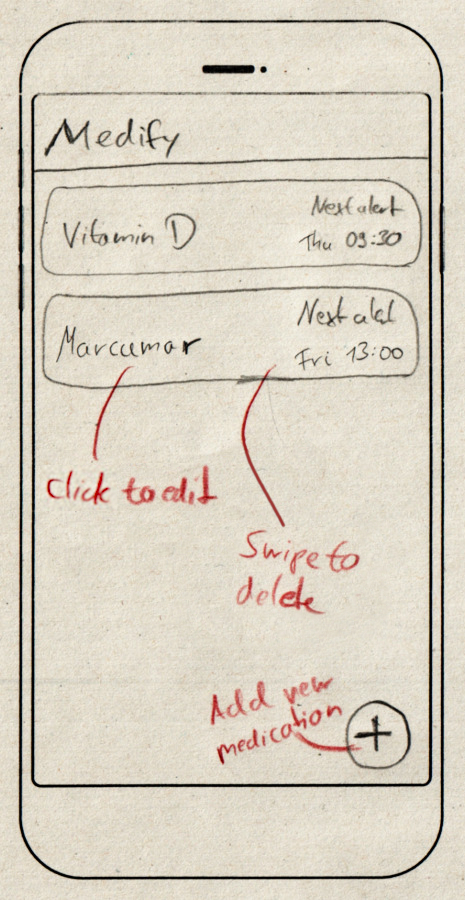
\includegraphics[width=0.4\linewidth]{images/mockup01}}
	\caption{Mockup of the main activity. Red annotations shall clarify the functionality of the elements.}
	\label{fig:mockup_main_activity}
\end{figure}

The mockup of the main activity is shown in Fig. \ref{fig:mockup_main_activity}. Every medication entry is
displayed in a list. The list entries include the names of the medication and the next time an alert is triggered.
The entries are clickable, in order to edit them. Swiping an entry shall remove it.
A button at the bottom of the screen enables the user to add a new medication entry.

\begin{figure}[pb]
	\centerline{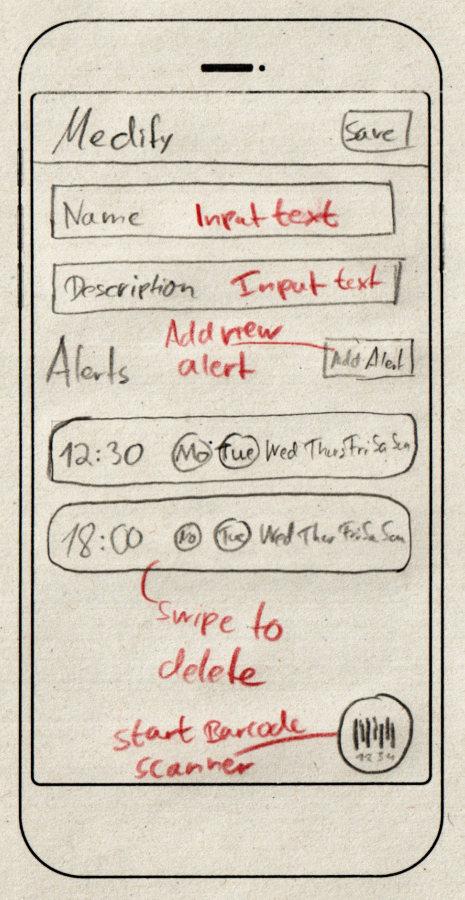
\includegraphics[width=0.45\linewidth]{images/mockup02}}
	\caption{Mockup of the form activity.}
	\label{fig:mockup_edit_activity}
\end{figure}

Fig. \ref{fig:mockup_edit_activity} displays the activity, when a new medication is to be added or an existing
one was selected to be edited. Two text input fields enables the user to specify the name and a description of 
the medication. A list is used to show all the alerts of the associated medication. The entries include the time
in a 24-hour notation and abbreviations of the weekdays. The selected weekdays shall be highlighted. Adding new 
alerts is handled by clicking a button above the list. Removing existing alerts is done by swiping the list entry.
Editing existing alerts is not provided. At the lower right part of the screen a floating button enables the user
to activate the GTIN/EAN--label scanner. A new activity shall start to handle the scanning of the label.
In order to save the medication entry, a button is presented in the upper right top of the screen. To cancel the
editing or adding operation, the system wide back-button in the navigation-buttons is to be used.

\section{Design decisions}

This section describes the design decision, which taken while developing the application.

\subsection{Database}

In order to implement the \textit{CRUD} operations, the package \textit{Room} by \cite{room} was used.
In an attempt to realize the data model in Fig. \ref{fig:entity_relationship_diagram}, the implemented model
needed to be altered.

\begin{figure}[H]
	\centerline{\includesvg[width=\linewidth]{uml_diagram}}
	\caption{UML diagram depicting the data model of the application.}
	\label{fig:uml_diagram}
\end{figure}

Fig. \ref{fig:uml_diagram} is the resulting UML diagram of the implemented data model. To achieve a \texttt{1:n}
relationship between the entities \texttt{Medication} and \texttt{AlertTimestamp} a helper class
\texttt{MedicationWithAlertTimestamps} was introduced. This way \textit{Room} is able to fetch a medication entry
and all its associated alerts. To abstract the data model structure from the controller and view, a
\texttt{ViewModel} was implemented to manage the database operations, and to offer the view a \texttt{LiveData}
representation of all medication entries.

An attentive reader might wonder, why the implementation contains a \texttt{1:n} relationship, when a single
\texttt{AlertTimestamp} class has also a list of \texttt{timestamps}. One might come to the conclusion, that a
\texttt{1:1} relationship be sufficient. Or even just the \texttt{Medication} class with an list attribute called
\texttt{timestamps}.

The decision was taken to implement this model the way as in Fig. \ref{fig:uml_diagram}, because a single
\texttt{AlertTimestamp} entry shall represent an alert at a specific time of the day, which can be repeated
at every given weekday. This results the \texttt{timestamps} attribute list having up to seven entries and no
more. In order to have multiple alerts on the same weekday, the \texttt{Medication} class can have multiple 
\texttt{AlertTimestamp} entries.

\subsection{Managing alerts}

To manage alerts the class \textit{AlarmManager} \cite{alarmmanager} was leveraged. This class enables the
application to run code at a specific time.

Every time a new medication entry is added, the \textit{AlarmManager} shall schedule new alarms. When a
medication is updated, the manager shall update the existing alarms, which are associated to the
medication. Deleting a medication, shall cancel the associated alarms. In order to ensure consistency, these
operations are included in the \texttt{ViewModel}. When the \texttt{ViewModel} is commissioned to alter the 
database, it also guarantees, that the scheduled alarms are consistent to the current database.

The specific time of the alert is provided as an Unix timestamp inside the \texttt{AlertTimestamp} class.
The scheduled code is a notification, which provides the user the name and the medication description.
Future revisions shall include a more attentive seeking alarm, like a ringtone which need to be canceled
by the user.

\subsection{Scanning GTIN/EAN--label}

Scanning the labels on products requires the application to obtain permissions to the camera. By using the package
\textit{code-scanner} \cite{barcode} the scanning is achieved. The scanning-process is started, by 
starting an activity containing an intent with a result-request. The started activity uses the package
\textit{code-scanner}. When a label is successfully registered, the activity sets the recognized GTIN/EAN--number
as the result and finishes. The parent activity receives this number and can continue processing it.

\subsection{API calls}

Having a GTIN/EAN--number, the application can try to fetch information about the product from an online database.
An open database is provided by \cite{eandatabase}. This host has a limited number of daily API calls and has a
narrow spectrum of products registered. However it is sufficient to showcase the functionality. To manage the API
calls, the package \textit{Retrofit} \cite{retrofit} is used. Unfortunately the responses from the database are not
in any common form, like \textit{JSON}. Therefore a custom parser was implemented to interpret the server response.

\subsection{User interface}

%\section{Results}
%
%\section{Conclusion}

\newpage\hfill\newpage %TODO
\begin{thebibliography}{00}	
	\bibitem{personaimg} P. Wang, ``This Person Does Not Exist,'' \textit{thispersondoesnotexist.com}, [Online]. Available: \url{https://thispersondoesnotexist.com/} [Accessed Dec. 17, 2021].

	\bibitem{storyboard} Clever Prototypes, LLC, ``Storyboard That,'' \textit{storyboardthat.com}, [Online]. Available: \url{https://www.storyboardthat.com/}. [Accessed Dec. 17, 2021].
	
	\bibitem{room} Google, LLC, ``Room - Android Developers,'' \textit{android.com}, [Online] Available: \url{https://developer.android.com/jetpack/androidx/releases/room/}. [Accessed Dec. 22, 2021].
		
	\bibitem{alarmmanager} Google, LLC, ``AlarmManager - Android Developers,'' \textit{android.com}, [Online]. Available: \url{https://developer.android.com/reference/android/app/AlarmManager}. [Accessed Dec. 22, 2021].

	\bibitem{barcode} Y. Budiyev, ``yuriy-budiyev/code-scanner: Code scanner library for Android, based on ZXing,'' \textit{github.com/yuriy-budiyev/code-scanner/}, [Online]. Available: \url{https://github.com/yuriy-budiyev/code-scanner/}. [Accessed Dec. 22, 2021].

	\bibitem{eandatabase} ``Open EAN Database - Datenbank und Produktbewertung,'' \textit{opengtindb.org}, [Online]. Available: \url{https://opengtindb.org/}. [Accessed Dec. 22, 2021].
	
	\bibitem{retrofit} Square, Inc., ``Retrofit,'' \textit{square.github.io/retrofit/}, [Online]. Available: \url{https://square.github.io/retrofit/}. [Accessed Dec. 22, 2021].
\end{thebibliography}

\end{document}

